\section{Auditor Extension} \label{sec:auditor}
Until now we have not verified whether a certificate chain is logged as promised
by any issued SCT.  Our base design can be extended to follow-up on inclusion
statuses rather than opting for cross-logging.  In terms of
the number of necessary changes, this extension is more significant when
compared to Section~\ref{sec:log}.  However, it does not require any log
modifications, and it entails additional ecosystem value by providing a
well-audited view of the CT landscape which is captured by the Tor consensus.
It is possible to detect internal inconsistency attacks within the Tor
network and omission attacks.  Trust in some logs is also shifted towards CT
auditors.

\subsection{Design Sketch} \label{sec:auditor:design}
Figure~\ref{fig:auditor} provides an overview of the extended design.  Tor
Browser submits presented SFOs probabilistically to CTRs that are selected at
random, and CTRs mix the submitted SFOs before any auditing takes place.  Here,
auditing refers to inclusion verification rather than cross-logging.  The moment
before an SFO is audited, it is shared with a CTR that takes on the role of a
\emph{watchdog}.  Unless the auditing CTR receives a timely inclusion proof and
acknowledges it to its watchdog, the SFO in question is reported to a CT
auditor.  Phase~1 remains unchanged, minor changes are needed in phase~2, and
major changes are required in phase~3 as well as the Tor consensus.  The
extra-info document also includes two additional metrics that are related to
flooding (Section~\ref{sec:log}).  Another prerequisite is existence of
CT auditors.

\begin{figure*}
    \centering
    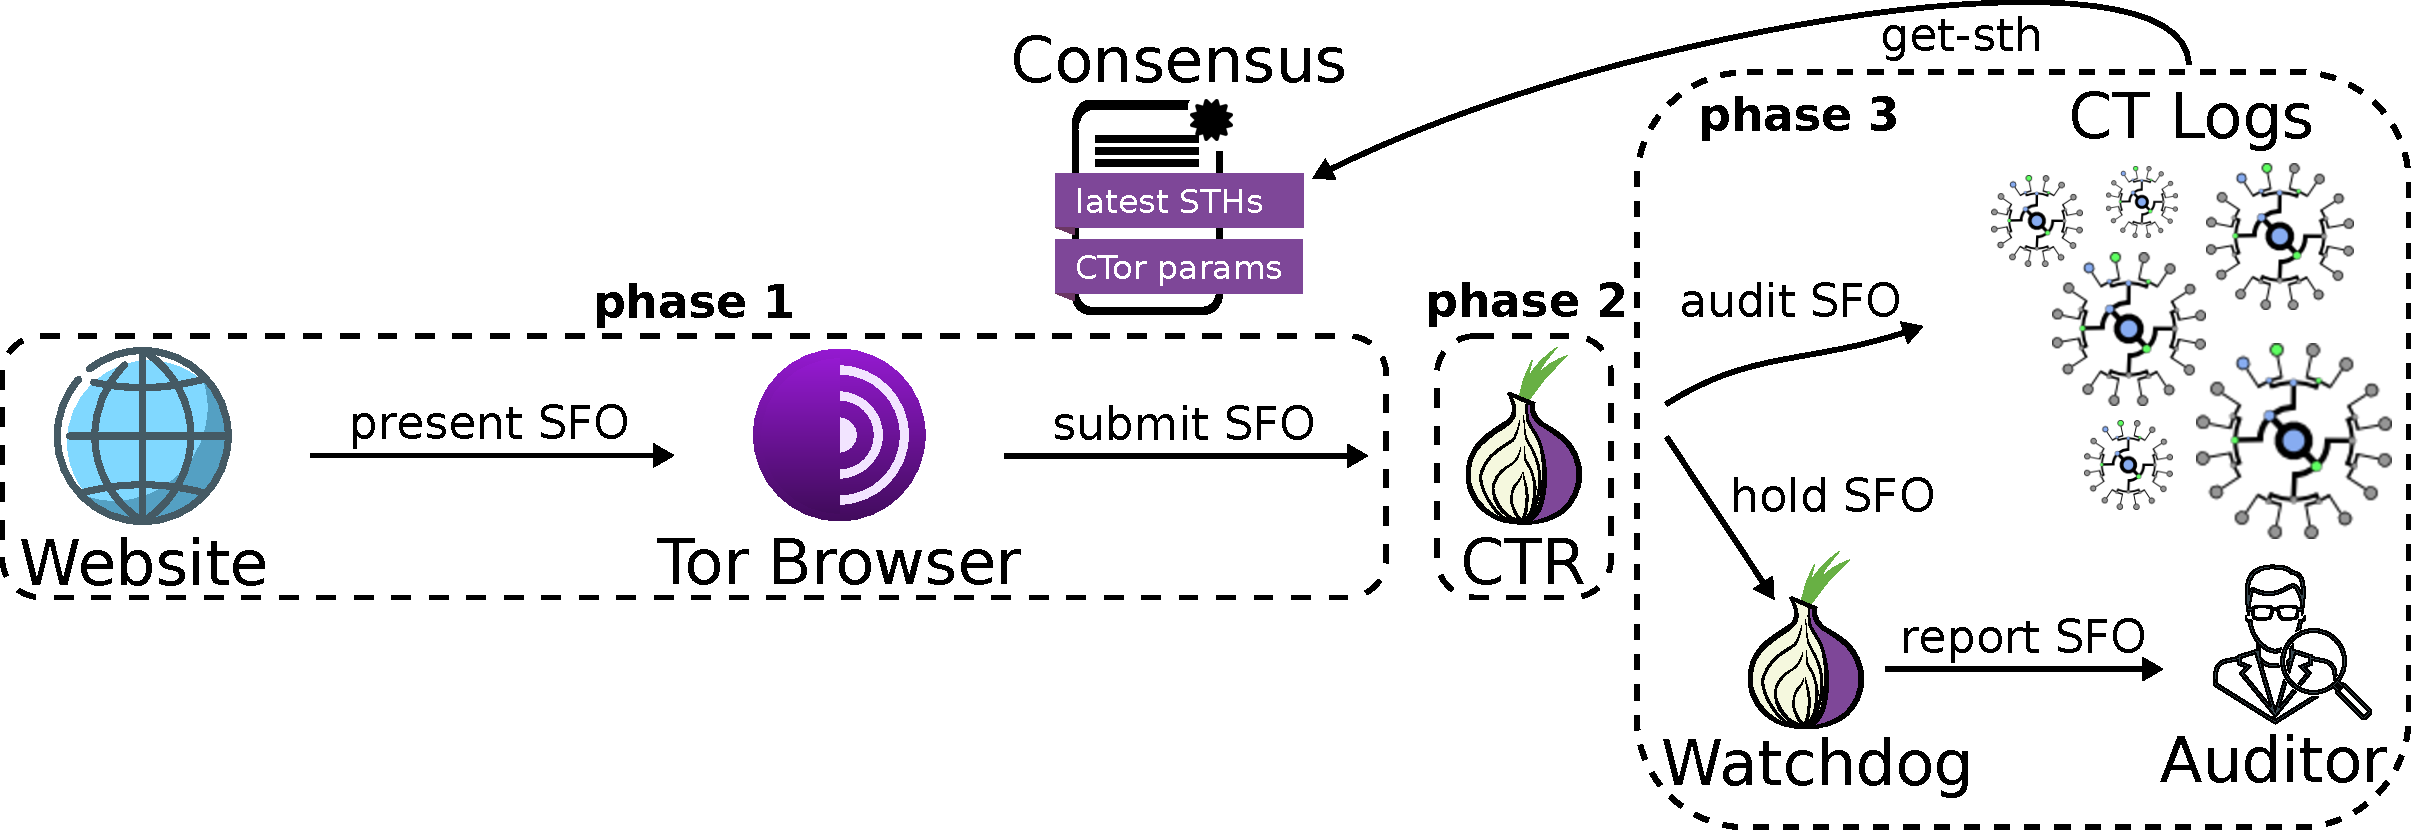
\includegraphics[width=0.85\textwidth]{img/design-auditor}
	\caption{The auditor extension to CTor, where cryptographic evidence of log
	omission can be collected without modification to CT logs. The extension
	changes the consensus to include the latest STHs from CT logs and makes
	phase 3 significantly more complex. CTRs in phase 3 now challenge logs to
	prove inclusion of certificates from SFOs, using other CTRs as
	``watchdogs'', ensuring that SFOs that are not provably correct are reported
	to trusted auditors.}
	\label{fig:auditor}
\end{figure*}

\subsubsection{Tor Consensus} \label{sec:auditor:design:consensus}
Tor's consensus should capture a fixed view of the CT landscape by publishing
STHs from all recognized logs.  A log is recognized if a majority of directory
authorities proposed a \texttt{ct-log-info} item, which contains a log's ID,
public key, base URL, MMD, and most recent STH.  Note that each directory
authority proposes its own STH, and agrees to use the most recent STH as
determined by timestamp.  Since CTRs verify inclusion statuses of SCTs
that Tor Browser accepts, the CT logs recognized by Tor Browser must be in
Tor's consensus.

Tor's directory authorities also majority-vote on \texttt{ct-auditor} items,
which pin base URLs and public keys of CT auditors that watchdogs contact in
case that any log misbehavior is suspected.  A watchdog triggers if the
\texttt{ct-watchdog-timeout} elapses without acknowledgment.  The following
auditor submission times-out if \texttt{ct-auditor-timeout} elapses.  These
items are determined similar to the \texttt{ct-query-timeout} in
Section~\ref{sec:base:consensus:params}.

\subsubsection{Phase~2: Storage} \label{sec:auditor:design:phase2}
A CTR cannot verify an SCT from an unrecognized log.
Step~\ref{enm:ctr-api:unrecognized} in Section~\ref{sec:base:phase2} should
therefore be updated so that unrecognized SCTs are discarded, stopping if no
SCT remains in the resulting SFO.  If an SFO is neither cached nor pending,
sample an SCT and note down the outcome and a corresponding
\texttt{audit\_after} timestamp using Figure~\ref{fig:audit-after}.  The
combination of SFO, sampled SCT outcome, and \texttt{audit\_after} timestamp is
stored in the pending buffer.  We already explained in Section~\ref{sec:log}
why it is important to take the log's MMD into account while computing
\texttt{audit\_after} timestamps.  The justification of sampling an SCT is
provided next in Section~\ref{sec:auditor:design:phase3}.

\subsubsection{Phase~3: Auditing} \label{sec:auditor:design:auditing}
The detailed auditing steps change to a large extent.  As such, we give a
detailed description from scratch instead.

\begin{enumerate}
	\item\label{enm:ctr:audit:backoff} Sample a uniform delay from
			$[0, \texttt{ct-backoff}]$,
		then schedule a timer and wait until that time elapsed.
	\item\label{enm:ctr:audit:log-circuit} Establish a new circuit and use it
		for all subsequent log connections.  Connect to the logs when needed.
	\item\label{enm:ctr:audit:watchdog-circuit} Establish a new three-hop
		circuit that ends at a randomly selected watchdog, i.e., another CTR.
	\item\label{enm:ctr:audit:loop} Enumerate the buffer of pending SFOs with
		regards to the sampled SCT and its associated STH:
		\begin{enumerate}
			\item\label{enm:ctr:audit:too-soon} Continue the loop if
				$\textrm{SFO}.\mathsf{audit\_after} > \mathsf{now}()$.
			\item\label{enm:ctr:audit:too-soon2} Continue the loop if
				$\textrm{SFO}.\mathsf{audit\_after} >
					\textrm{STH}.\mathsf{timestamp}$.
			\item\label{enm:ctr:audit:watchdog} Submit $s$ to the
				watchdog selected in step~\ref{enm:ctr:audit:watchdog-circuit}.
			\item\label{enm:ctr:audit:challenge} Use \texttt{ct-query-timeout}
				and $\textrm{STH}.\mathsf{treesize}$ to set a timer and
				challenge the log to prove inclusion.
				\begin{itemize}
					\item On valid proof: send an acknowledgment to the
						watchdog, then cache $s$ and discard it.
					\item On any other outcome: discard $s$ and break.
				\end{itemize}
		\end{enumerate}
	\item\label{enm:ctr:audit:teardown} Close all opened circuits and go back to
		step~\ref{enm:ctr:audit:backoff}.
\end{enumerate}

Each auditing instance uses a single watchdog, which takes on the responsibility
of reporting suspected log misbehavior on any other outcome than valid inclusion
proof.  It is motivated to use a watchdog because the attacker learns which
CTR audits an SFO, and could likely take actions to intervene while the CTR
waits for \texttt{ct-submit-timeout} to trigger (see
Section~\ref{sec:ext-auditor:analysis}).  A watchdog's behavior is to listen for
SFO submissions on a dedicated endpoint, and submit them to random CT auditors
that are pinned in the Tor consensus if no timely acknowledgments are received.
If an auditor is unavailable as indicated by timeouts, resubmit later on.

Note that an SFO's sampled SCT is not audited before the log's MMD elapsed
\emph{and} there is an STH in the Tor consensus that captures it.  It is
sufficient for CTRs to verify the inclusion status of a single SCT:
	a rational attacker is the issuer of all SCTs, and
	does not intend to hold its promises of merging in \emph{any} CT log.
As such, we merely need to suspect omissions and then let CT auditors inspect
all SCTs in the reported SFOs.

\subsubsection{Phase~3: Auditor} \label{sec:auditor:design:auditor}
An announced auditor is expected to accept SFOs at a dedicated endpoint,
endeavoring to validate the inclusion status of each SCT with regards to the
first STH in the Tor consensus that elapsed the log's MMD.  If a log appears to
function correctly except for some evidence that cannot be
resolved despite multiple attempts that span a given time period, it is
paramount that the auditor software alerts its operator who can investigate
the issue further before submitting a full report to the CT-policy mailing list.
Cases of misbehavior in detail:
\begin{itemize}
	\item If the log fails to provide a valid inclusion proof for an SCT with
		regards to the first applicable STH in the Tor consensus
		(certificate omission).
	\item If the log fails to provide a valid consistency proof between two
		STHs in the Tor consensus
		(split-view).
	\item If a published STH is future-dated or backdated more than an MMD
		(general log misbehavior).
	\item If a log ignores some CTRs (uptime misbehavior).
\end{itemize}

An unresponsive log can be suspected by observing the watchdog report frequency,
and possibly confirmed by querying the log in question from different vantage
points.  Among other extra-info metrics that go beyond received and deleted
SFO-bytes, it could be valuable to publish the extent to which CTR-to-log
interactions fail.

While not within our threat model, we do encourage the announced auditors to
verify that STHs in the Tor consensus are consistent with external views of the
CT landscape.  For example, operate an STH pollination~\cite{nordberg} endpoint
and fetch STHs actively from many diverse vantage points using Tor, VPN
services, DoH resolvers, and RIPE Atlas (to mention a few low-cost options).
This goes back to the point of general ecosystem value.

\subsection{Security Analysis} \label{sec:auditor:design:analysis}
% MISC notes
% - Network-wide flush, detectable but hard to attribute
% - Requires new reliable auditor software
% - Bit more bandwidth due to watchdog.  The overhead, when compared to log a
% log extension, is sending an SCT hash and receiving a proof (2-3KiB).
